%!TEX root = ../thesis.tex

\subsection{経路計画とは}

\begin{figure}[hbtp]
  \centering
 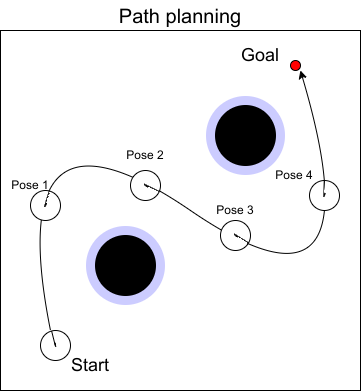
\includegraphics[keepaspectratio, scale=0.8]
      {images/png/PathPlanning.drawio.png}
 \caption{Path planning}
 \label{Fig:PathPlanning}
\end{figure}

経路計画は前述したように,ロボットがどのように通るかを計画することである.経路計画では,
ロボットの姿勢と位置,スタートからゴールまでにある障害物が考慮されたスタート地点からゴールまでの最短な経路が計画される.
計画された経路はロボットが通るべき位置,そのときに取るべき姿勢とその地点を通る順番の3つの条件からなる
複数の点の集合であると言うことができる.

Fig.\ref{Fig:PathPlanning}は経路計画のイメージ図である.黒と青の円で表されているのが障害物であり,
円と線分で表されているのがロボットである.線分の向きがロボットの姿勢を表している.
Fig.\ref{Fig:PathPlanning}のように経路計画では,ロボットの姿勢と位置が順番に指定される.
\newpage
